\documentclass{beamer}
\usetheme{Copenhagen}
\usepackage{hyperref}
\usepackage[T1]{fontenc}
% \usepackage{enumitem}
\usepackage{xcolor}
\usepackage{pifont}

% other packages
\usepackage{latexsym,amsmath,xcolor,multicol,booktabs,calligra}
\usepackage{graphicx,pstricks,listings,stackengine}

% Define custom symbols
\newcommand{\cmark}{\textcolor{green!70!black}{\ding{51}}} % green tick
\newcommand{\xmark}{\textcolor{red}{\ding{55}}}            % red cross



\author{Andrei Ilin}
\title{Timing Anomaly through Branch Prediction}
% \subtitle{Cospa group meeting}
\subtitle{Supervised by Lionel Rieg, Florian Brandner and Mihail Asavoae}
\institute{Université Grenoble Alpes}
\date{23 June 2025}
\usepackage{USTC_beamer}

% \renewcommand{\familydefault}{\rmdefault}

% defs
\def\cmd#1{\texttt{\color{red}\footnotesize $\backslash$#1}}
\def\env#1{\texttt{\color{blue}\footnotesize #1}}
\definecolor{deepblue}{rgb}{0,0,0.5}
\definecolor{deepred}{rgb}{0.6,0,0}
\definecolor{deepgreen}{rgb}{0,0.5,0}
\definecolor{halfgray}{gray}{0.55}

\lstset{
    basicstyle=\ttfamily\small,
    keywordstyle=\bfseries\color{deepblue},
    emphstyle=\ttfamily\color{deepred},  
    stringstyle=\color{deepgreen},
    numbers=left,
    numberstyle=\small\color{halfgray},
    rulesepcolor=\color{red!20!green!20!blue!20},
    frame=shadowbox,
}

\includeonlyframes{current}
\begin{document}

% Define custom item styles


% \kaishu
\renewcommand{\figurename}{Fig.}

% logo
\begin{frame}
    \titlepage
    \begin{figure}[htpb]
        \begin{center}
            
\includegraphics[width=0.2\linewidth]{pic/logo-uga.png}\hspace{1.5cm}
            
\includegraphics[width=0.2\linewidth]{pic/logo-verimag.png}\hspace{1.5cm}
            
\includegraphics[width=0.2\linewidth]{pic/logo-INP.png}
        \end{center}
    \end{figure}
\end{frame}
% \TODO fix title

\begin{frame}
    \tableofcontents[sectionstyle=show,subsectionstyle=show/shaded/hide,subsubsectionstyle=show/shaded/hide]
\end{frame}

\section{Introduction}

\begin{frame}{Critical Real-Time Systems}
    \begin{columns}
        \begin{column}{0.5\textwidth}
            \begin{block}{Can be found in:}
                \begin{itemize}
                    \item Cars 
                    \item Planes
                    \item Life-supporting equipment
                \end{itemize}
            \end{block}
        \end{column}

        \begin{column}{0.5\textwidth}
            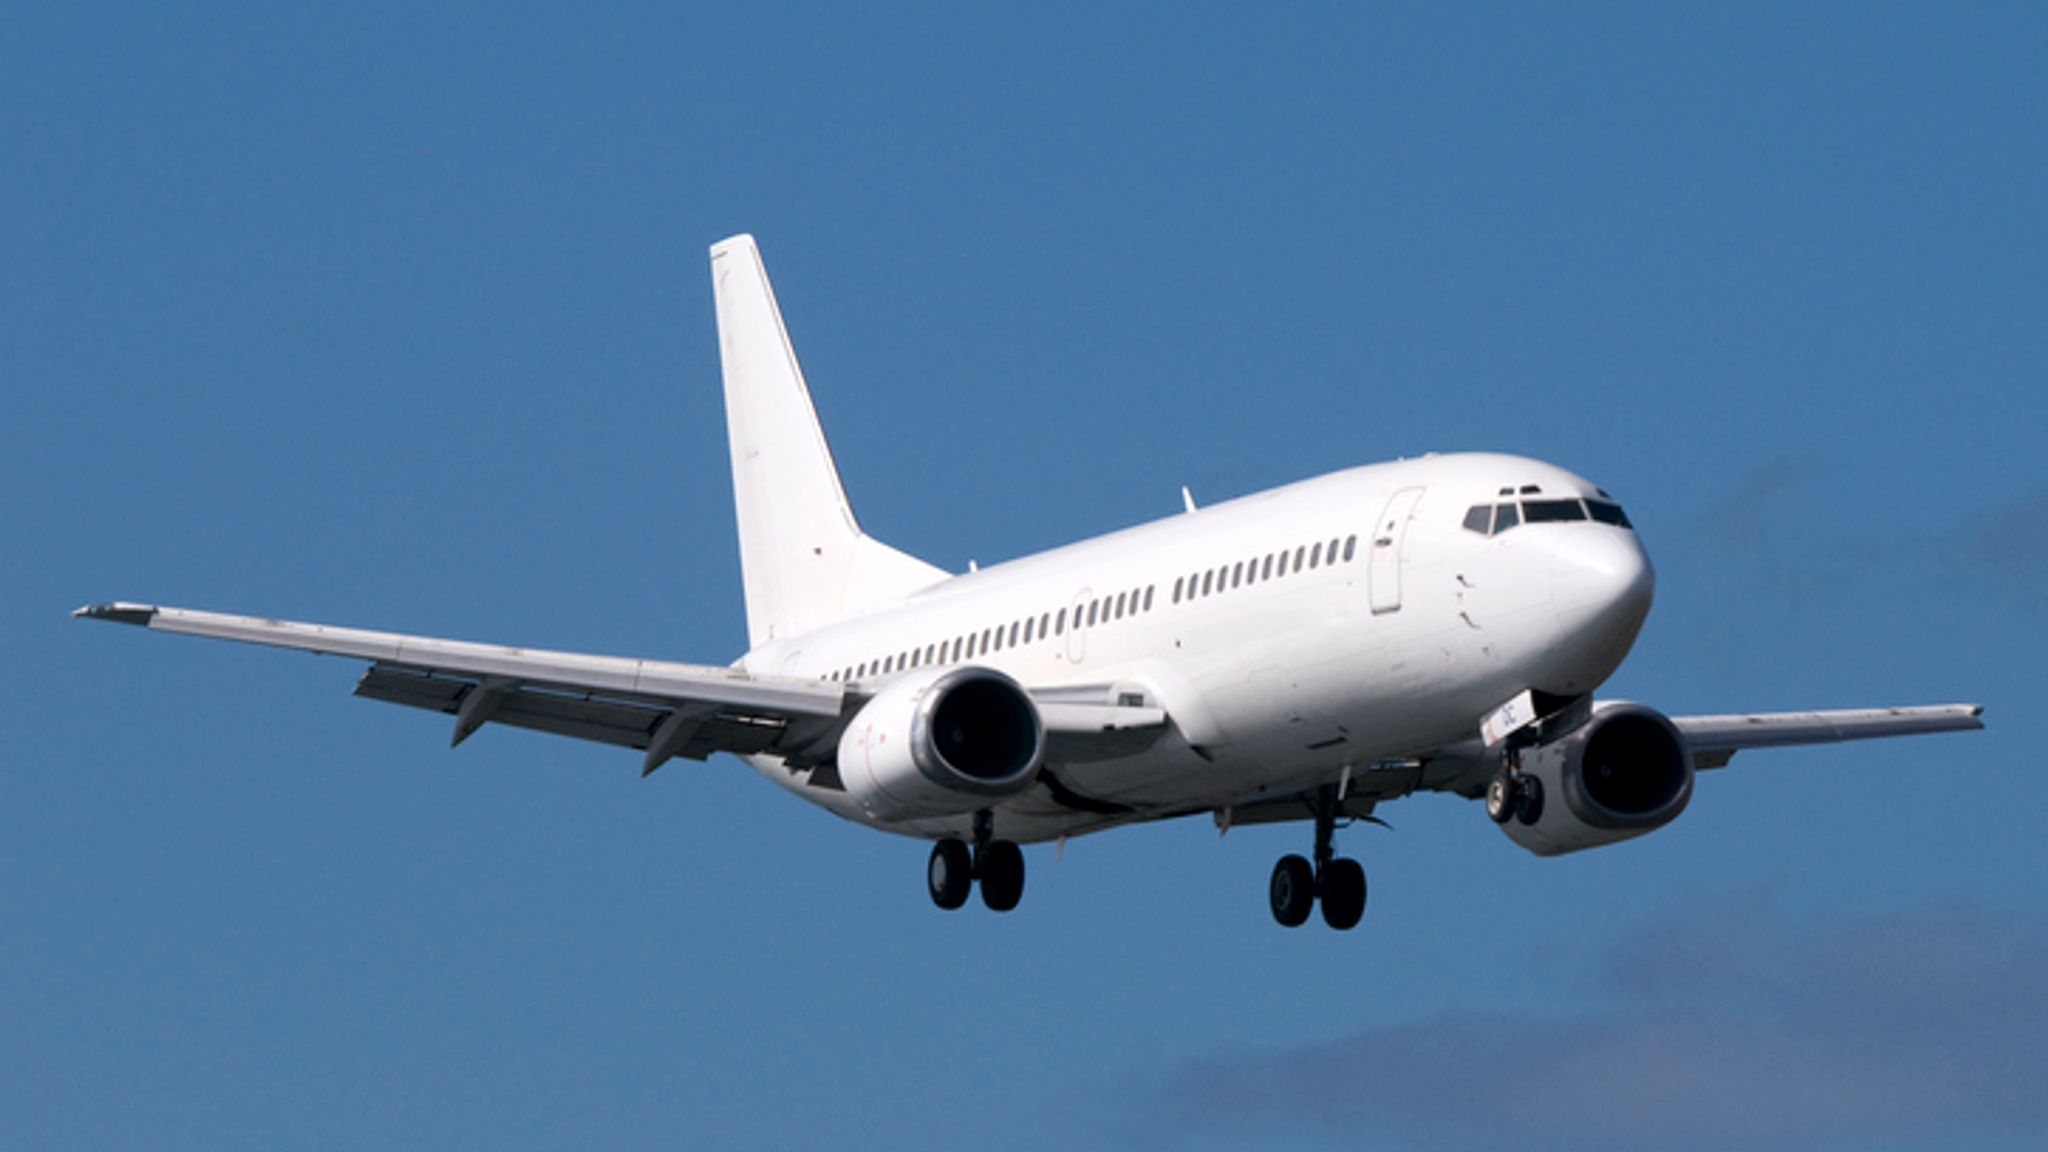
\includegraphics[width=\textwidth]{pic/plane.png}
        \end{column}
    \end{columns}

    \hfill \break
    \hfill \break

    Strict timing requirements for the programs.

    \begin{exampleblock}{Example}
        Car break system that must respond in 5 ms.
    \end{exampleblock}
    
\end{frame}

% Ex: break respond time...

\begin{frame}{WCET Analysis}
    \begin{columns}
        
    \column{0.4\textwidth}

    \textbf{W}orst \textbf{C}ase \textbf{E}xecution \textbf{T}ime Analysis:
    \begin{itemize}
        \item Hardware + Software
        \item Upper bound for execution time?
    \end{itemize}


    \begin{block}{}
        Analysis is split into multiple stages and uses simplifications.
    \end{block}

    \column{0.6\textwidth}

    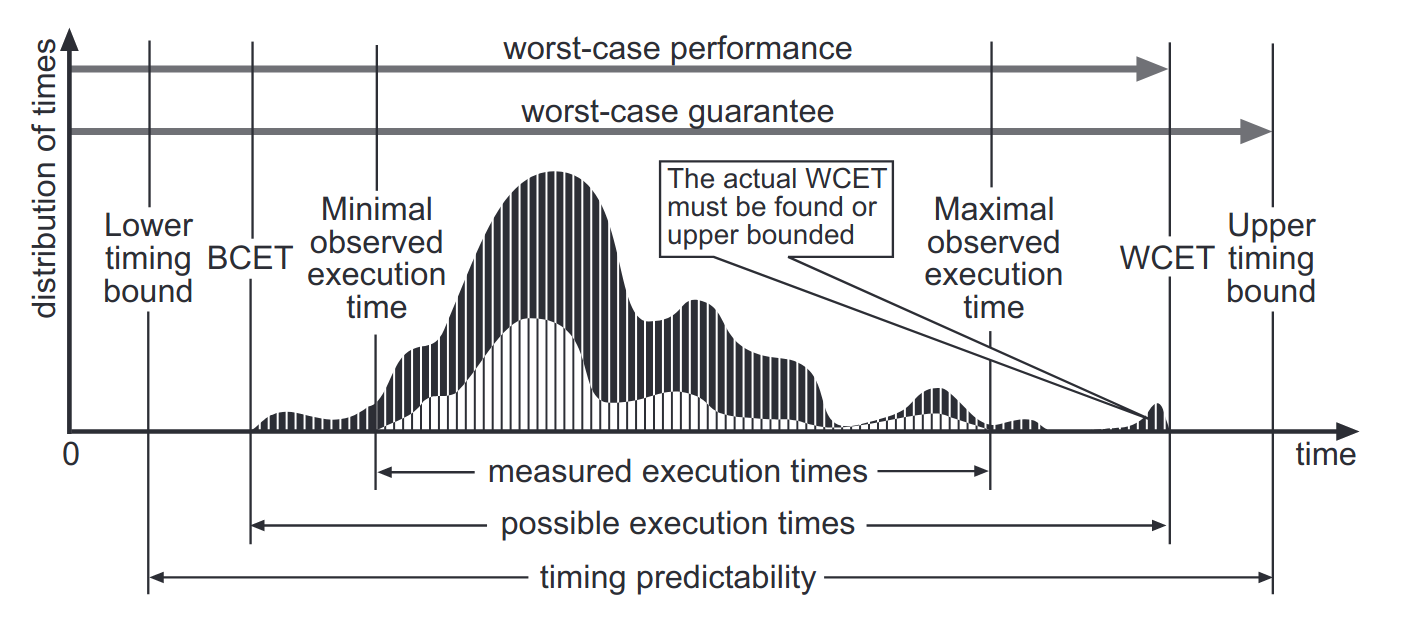
\includegraphics[width=1\textwidth]{pic/timing-distribution.png}

    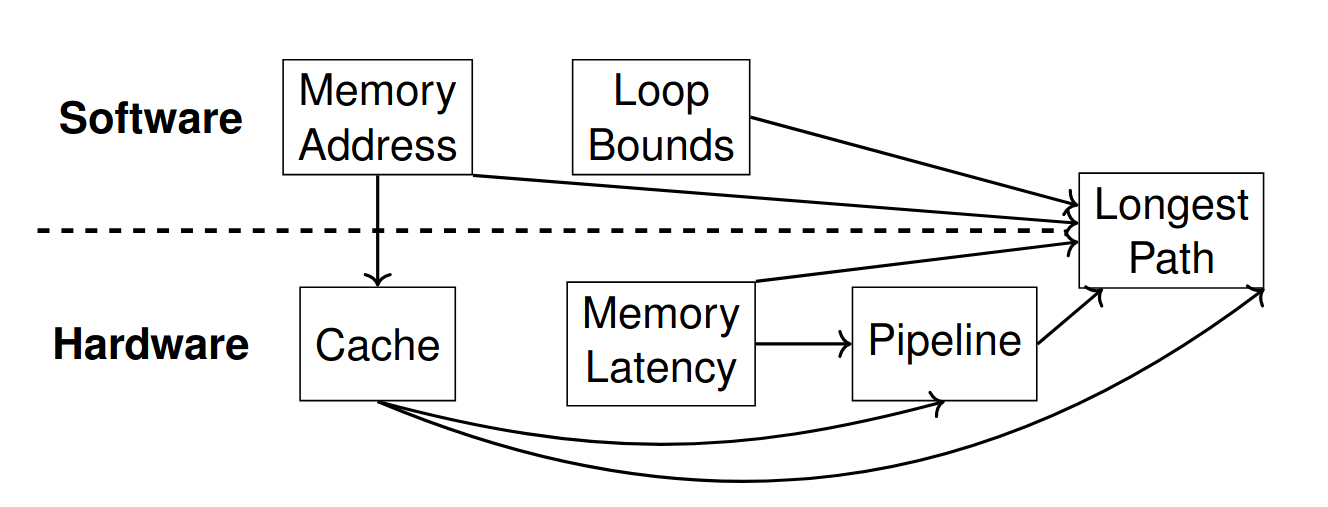
\includegraphics[width=1\textwidth]{pic/wcet-deps.png}

    \end{columns}
\end{frame}

% Animate distribution?
% Say: overestimation, simplification 
% Full system too complicated -> split anal. -> ASS.: sys are composable
% Not all are composable, thus TA


\begin{frame}{Timing Anomalies}
    \begin{block}{Timing Anomaly (TA)}
        When a local speedup leads to a global slowdown.
    \end{block}

    \begin{exampleblock}{Example}
        Faster completion of $A$ leads to a slowdown of the whole trace. 
    \end{exampleblock}

    \begin{columns}
    \column{0.4\textwidth}
        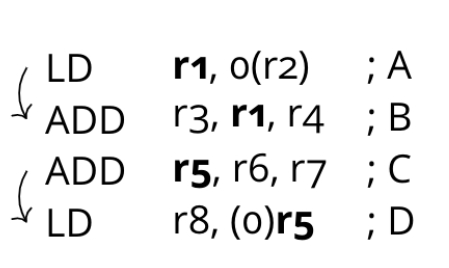
\includegraphics[width=1\textwidth]{pic/first-TA-ex-input.png}
    \column{0.6\textwidth}
        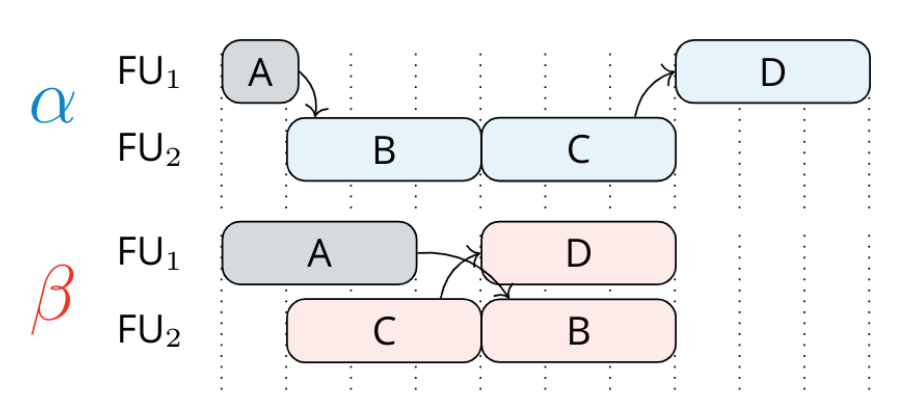
\includegraphics[width=1\textwidth]{pic/first-TA-ex-trace.png}
    \end{columns}
\end{frame}

% 

\section{Hardware}

\begin{frame}{OoO Multiscalar Pipeline}
    Processor:
    \begin{itemize}
        \item \textbf{Pipelined:} Divided into consecutive stages
        \item \textbf{Superscalar:} Fetch multiple instruction in the same time
        \item \textbf{Out-of-Order:} Execution order dictated by scheduling policy
    \end{itemize}


    \begin{columns}
    \column{0.5\textwidth}
        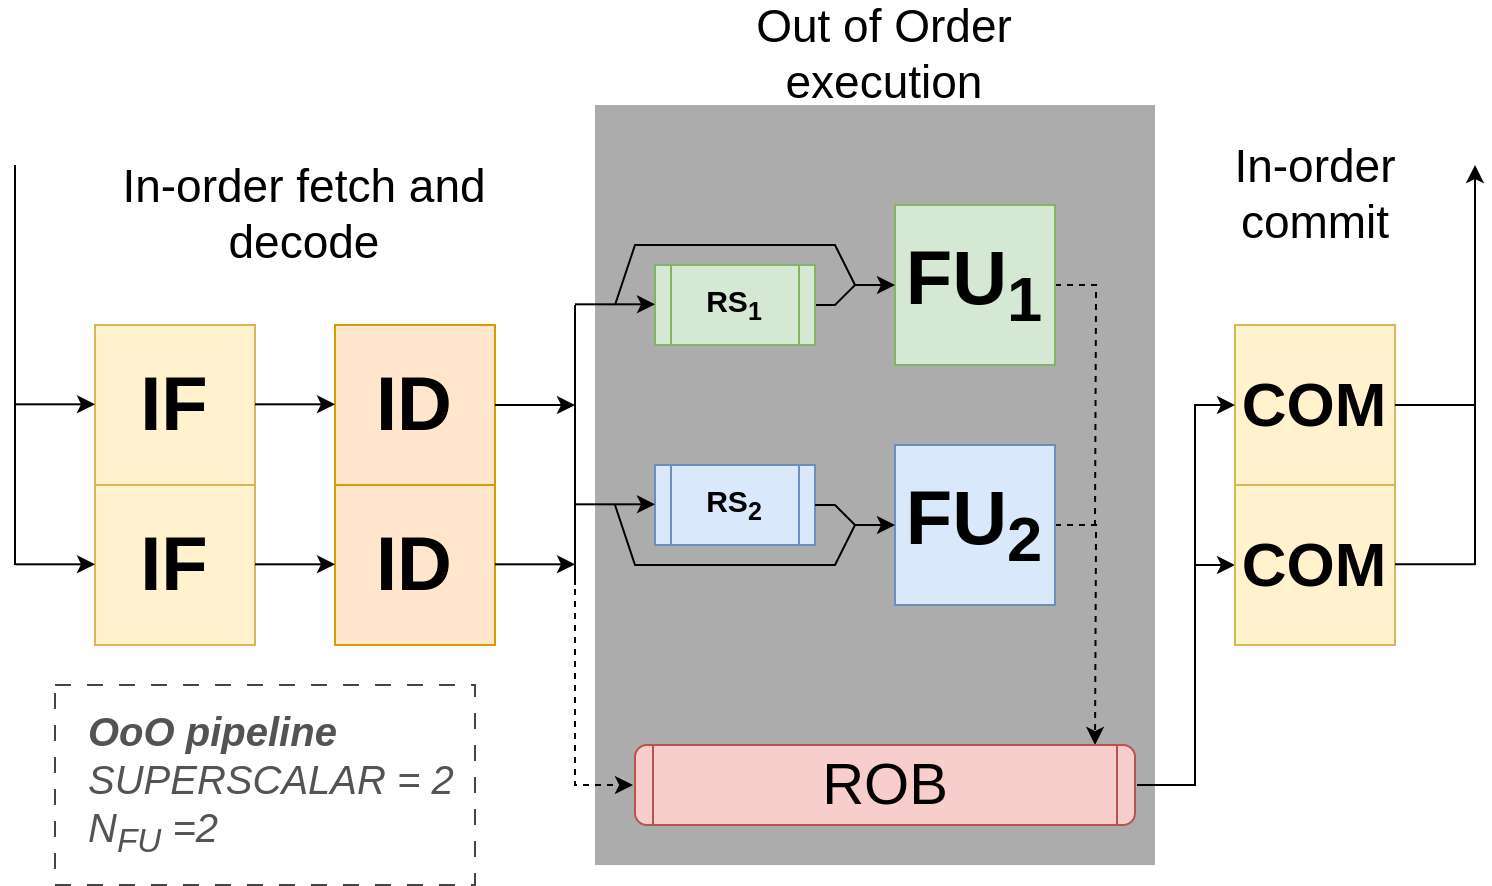
\includegraphics[width=\textwidth]{pic/pipeline.png}
    \column{0.5\textwidth}
        \includegraphics<1>[scale=0.14]{pic/multiscalar-demo-1.png}
        \includegraphics<2>[scale=0.14]{pic/multiscalar-demo-2.png}
        \includegraphics<3>[scale=0.14]{pic/multiscalar-demo-3.png}
        \includegraphics<4>[scale=0.14]{pic/multiscalar-demo-4.png}
    \end{columns}

\end{frame}

% Explain ROB: keep track of dependencies, each instr = 1 entery in ROB, when enters
% No TA: just one trace: some arrows clarif.


\begin{frame}{Branch Prediction}
    
    \begin{itemize}
        \item<1-3> Branch target unknown until branch is resolved.
        \item<2-3> Predict next address and execute speculatively.
        \item<3> Misprediction detected $\rightarrow$ start fetching the correct branch
    \end{itemize}

    
    \includegraphics<1>[scale=0.17]{pic/bp-demo-no.png}
    \includegraphics<2>[scale=0.17]{pic/bp-demo-correct.png}
    \includegraphics<3>[scale=0.17]{pic/bp-demo-incorrect.png}

\end{frame}

% \TODO Show first without BP: we have to wait; Animation


\begin{frame}{Branch Prediction: possible implementations}
    \begin{columns}
    \column{0.5\textwidth}

    \begin{block}{Additional Hardware}
        \begin{itemize}
            \item Pattern History Table (PHT)
            \item Branch Target Buffer (BTB)
        \end{itemize}
    \end{block}

    \begin{exampleblock}{Example: 2-bit counter}
        For each branch store a 4-state automaton in PHT
    \end{exampleblock}

    \column{0.5\textwidth}

    \begin{block}{Strategies}
        \textbf{Static:} always take, never take, take backwards. \\        
        \textbf{Dynamic:} 
        \begin{itemize}
            \item 1 or 2-Bit Counter
            \item Global or Local History
            \item Global share
        \end{itemize}
        and more...
    \end{block}

    \end{columns}

    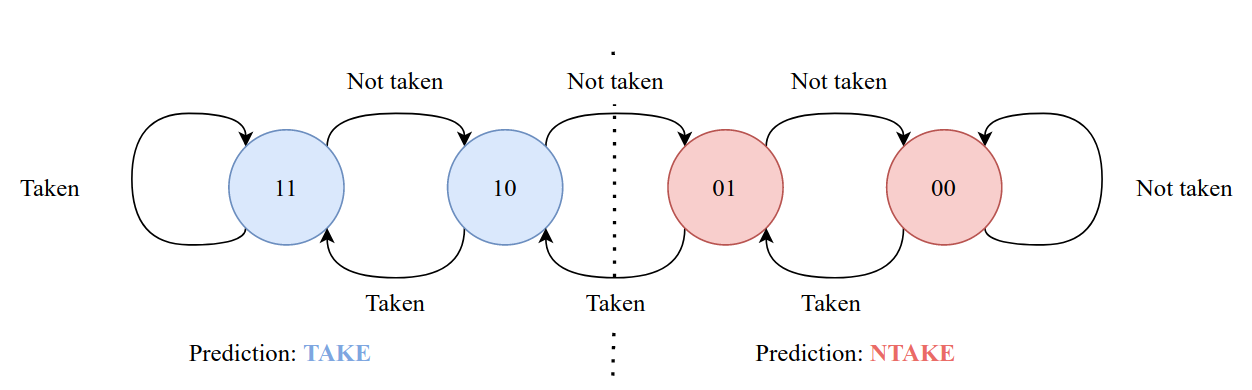
\includegraphics[width=0.9\textwidth]{pic/two-bit-counter.png}
\end{frame}

% Not structured well
% 2-bit coutner = 2 incorrect predictions to change
% PHT - remember past branch
% BTB - too remember the target

\section{Timing Anomalies}

\begin{frame}{Formal Definition?}
    \textbf{How do we formally define a TA?}

    \only<1>{
        \begin{block}{Many existing definitions}
        \begin{itemize}
                \item Step Heights (by Gebhard et al.)
                \item Step-functions Intersections (by Cassez et al.)
                \item Component Occupation (by Kirner et al.)
                \item Instruction Locality (by Reineke et al.)
                \item Event Time Dependency Graph (by Binder et al.)
            \end{itemize}
        \end{block}
    }

    \only<2>{
        \begin{block}{Many existing definitions}
        \begin{itemize}
                \item \textbf{Step Heights (by Gebhard et al.)}
                \item \textbf{Step-functions Intersections (by Cassez et al.)}
                \item Component Occupation (by Kirner et al.)
                \item Instruction Locality (by Reineke et al.)
                \item \textbf{Event Time Dependency Graph (by Binder et al.)}
            \end{itemize}
        \end{block}
    }
    
\end{frame}

% Key ideas of defs?

\begin{frame}{Step Heights by Gebhard et al.}
    \begin{block}{Definition}
        TA = instruction latency (compared to previous instr.) smaller, global time greater
    \end{block}

    \includegraphics<1>[width=\textwidth]{pic/step-height-good.png}

    \begin{alertblock}<2>{Counterexample!}
        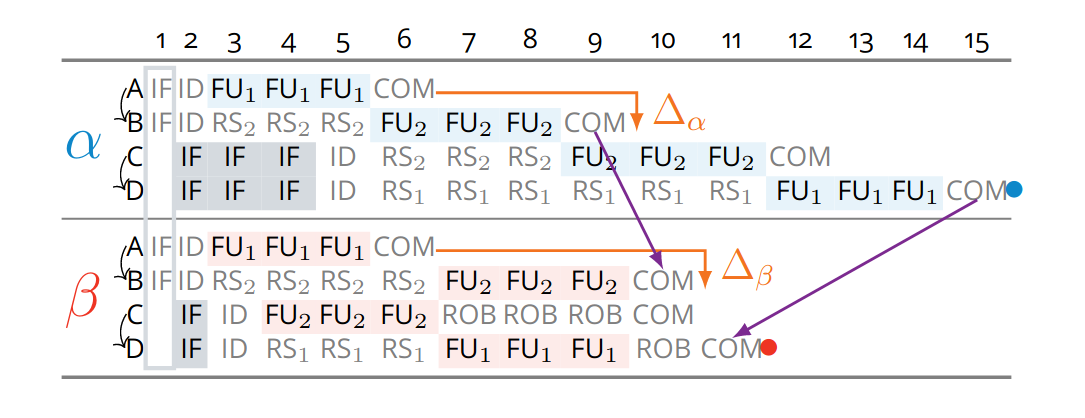
\includegraphics[width=0.7\textwidth]{pic/step-height-bad.png}
    \end{alertblock}
\end{frame}
% Be simpler: arrow in diff. directions
% Counterexamples: 2 lines cross, but no TA!
% Swap coutnerexamples !!!


\begin{frame}{Step Function Intersections by Cassez et al.}
    \begin{block}{Definition}
        TA = one instruction finishes earlier than in alternative trace, the other later than in alternative trace
    \end{block}

    \only<1>{
        \begin{columns}
        \column{0.8\textwidth}
            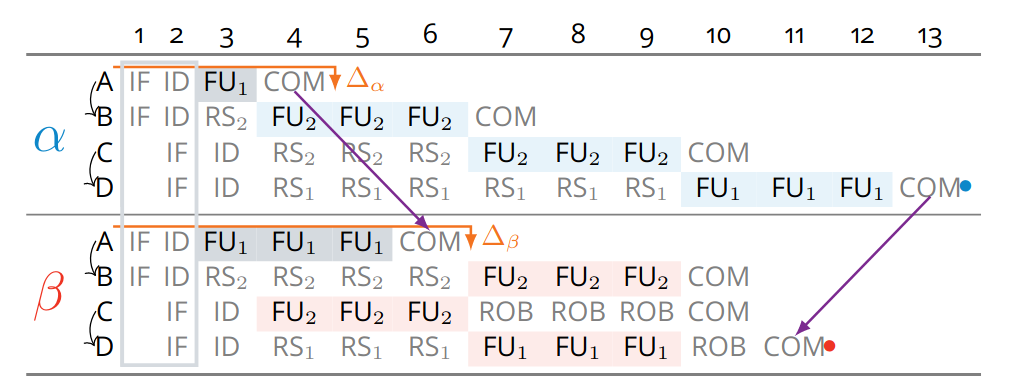
\includegraphics[width=\textwidth]{pic/step-height-good.png}
        % \column{0.4\textwidth}
        %     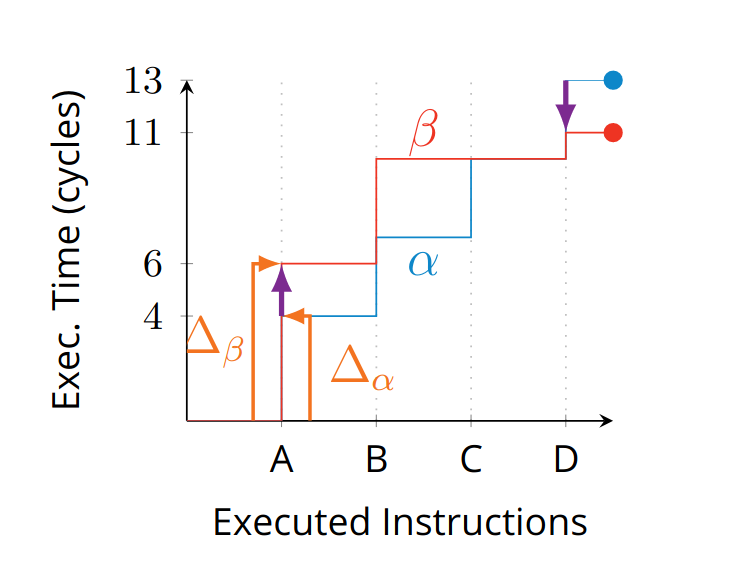
\includegraphics[width=\textwidth]{pic/step-functions.png}
    \end{columns}
    }
    
    \only<2>{
        \begin{alertblock}{Counterexample!}
            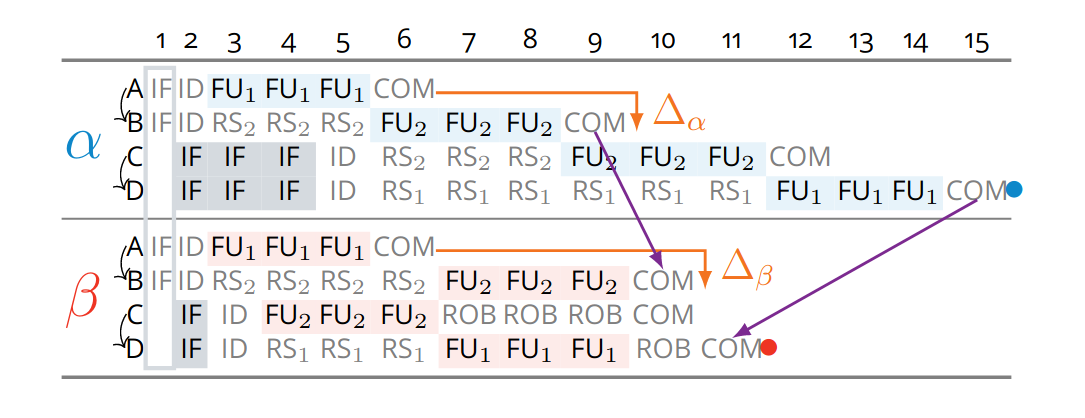
\includegraphics[width=0.9\textwidth]{pic/step-functions-bad.png}
        \end{alertblock}
    }   
\end{frame}
% Idea of rotating the exec. pattern
% Counterexample: step function !!
% Is example correct?

\begin{frame}{Event Time Dependency Graph by Binder et al.}
    \begin{block}{3 Components}
        \only<1> {
            \begin{enumerate}
                \item Variation
                \item Slowdown
                \item Causality
            \end{enumerate}
        }
        \only<2> {
            \begin{enumerate}
                \item \textbf{Variation} in latency
                \item Slowdown
                \item Causality
            \end{enumerate}
        }
        \only<3> {
            \begin{enumerate}
                \item Variation in latency
                \item \textbf{Slowdown} in delay end of variation $\rightarrow$ later event
                \item Causality
            \end{enumerate}
        }
        \only<4> {
            \begin{enumerate}
                \item Variation in latency
                \item Slowdown  in delay end of (variation $\rightarrow$ later event)
                \item \textbf{Causality} link = event $X$ cannot be earlier because of $Y$
            \end{enumerate}
        }
    \end{block}

    \includegraphics<1>[scale=0.17]{pic/binder-def-1.png}
    \includegraphics<2>[scale=0.17]{pic/binder-def-2.png}
    \includegraphics<3>[scale=0.17]{pic/binder-def-3.png}
    \includegraphics<4>[scale=0.17]{pic/binder-def-4.png}
\end{frame}

% Causality - why do we need it? In counterex no relation between source and TA
% Causality only in one trace

\begin{frame}
    \begin{block}{Goal}
        Develop a consistent TA definition applicable for branch prediction.
    \end{block}

    \begin{itemize}
        \item \textbf{Question 1} Can timing anomaly be caused by branch prediction?
        \item \textbf{Question 2} Can we extend the existing Binder's definition?
        \item \textbf{Question 3} Do we cover all the aspects of branch prediction?
    \end{itemize}

\end{frame}
% + subquestions
% can we extend causality-based def?
% how to do that?

\section{Contribution}

\begin{frame}{Research Plan}
    \begin{enumerate}
        \item Create a tool for automatic example generation.
        \item Generate some candidate scenarios.
        \item Try to adapt definition on them.
        \item Find new scenarios to verify the definition.
    \end{enumerate}
\end{frame}
% Too long. Make it more visual
% TLA problems, C++ problems, compare

\begin{frame}{Tool Implementation}
    % \begin{alertblock}{TLA+ implementation}
    %     Is slow. 2-3 seconds to generate a single example.
    % \end{alertblock}

    % \begin{itemize}
    %     \item Written in C++.
    %     \item Simple and flexible input format.
    %     \item Supports speculative execution.
    %     \item Faster than TLA$+$ implementation (ms instead of seconds).
    %     \item 3 operation modes:
    %     \begin{enumerate}
    %         \item Interactive manual mode.
    %         \item Randomized search.
    %         \item State space exploration.
    %     \end{enumerate}
    %     \item Lacks formal gurantees
    % \end{itemize}

    

    \begin{columns}
        \column{0.5\textwidth}
        \begin{exampleblock}{Existing TLA$^+$ framework}

            \begin{itemize}
                \item[\xmark] Slow: 2-3 seconds for single example
                \item[\xmark] No branch and speculation support
                \item[\xmark] Lengthy input format 
                \item[\cmark] Formal guarantees
            \end{itemize}

            
        \end{exampleblock}

        \column{0.5\textwidth}
        \pause
        \begin{exampleblock}{Our C++ framework}
            \begin{itemize}
                \item[\cmark] Fast: a few ms per example
                \item[ ]
                \item[\cmark] Traces with speculation
                \item[ ] 
                \item[\cmark] Refined consize input format
                \item[\xmark] Harder to specify properties
            \end{itemize}
        \end{exampleblock}
    \end{columns}

\end{frame}
% Better to do a comparison: 2 columns, pros and cons
% We starte by doing TLA+ implem., but then...
% Animation

\begin{frame}{Input Format}

\begin{itemize}
    \item Each branch instruction is followed by \textbf{misprediction region} -- sequence of instruction representing the wrong branch.
    \item A pair of traces is generated from a single input.
\end{itemize}
% How the input format is new
% Meaning of indentation
% Explain squash on diagram, what diagram mean
% Write: some instr. disappera, so harder to compare

\begin{columns}
    \column{0.4\textwidth}
        \begin{tabular}{rr|ccc}
         &  & Res & Dep. & Lat. \\ \hline
        \textit{A} &  & FU1 &  & $4$ \\
        \textit{*B} &  & FU2 & $\{A\}$ & $1$ \\
        & \textit{C} & FU2 &  & $4$ \\
        & \textit{D} & FU2 &  & $4$ \\
        \textit{E} &  & FU2 &  & $4$ \\
        \end{tabular}

    \column{0.6\textwidth}
        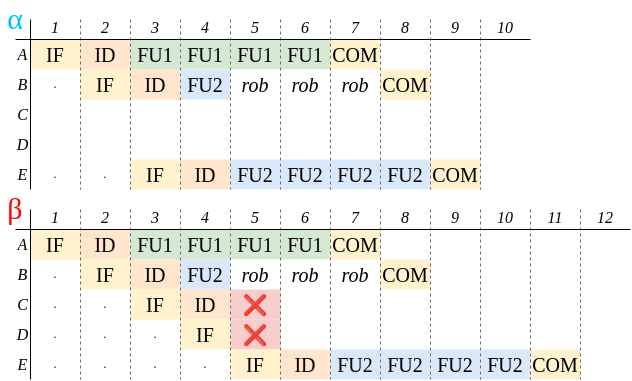
\includegraphics[width=\textwidth]{pic/mispred-intro.png}
\end{columns}

\end{frame}
% \TODO add mispred notation

\begin{frame}{Branch TA}
    Correct prediction leads to a longer execution time.

    \includegraphics<1>[scale=0.13]{pic/simple-branch-ta-analyzed-1.png}
    \includegraphics<2>[scale=0.13]{pic/simple-branch-ta-analyzed-2.png}
    \includegraphics<3>[scale=0.13]{pic/simple-branch-ta-analyzed-3.png}
    \includegraphics<4>[scale=0.13]{pic/simple-branch-ta-analyzed-4.png}

    \begin{exampleblock}{Where is latency?}
        \only<2->{Between "branch prediction" and "correct branch taken" events.}
    \end{exampleblock}

    \only<3->{No need to adapt delay and causality.}

    
\end{frame}
% Question: can we fit Binder's def?
% ...and this is the answer
% Why latency
% TODO: animation

% Viusal example
% Names for assumtions!
% Restructure: introduce assumption with examples
% Put the input format!

% \begin{frame}{Early FU Release}
%     \begin{itemize}
%         \item \textbf{Assumption 1} does not hold.
%         \item \textbf{Assumption 2} holds.
%     \end{itemize}
%     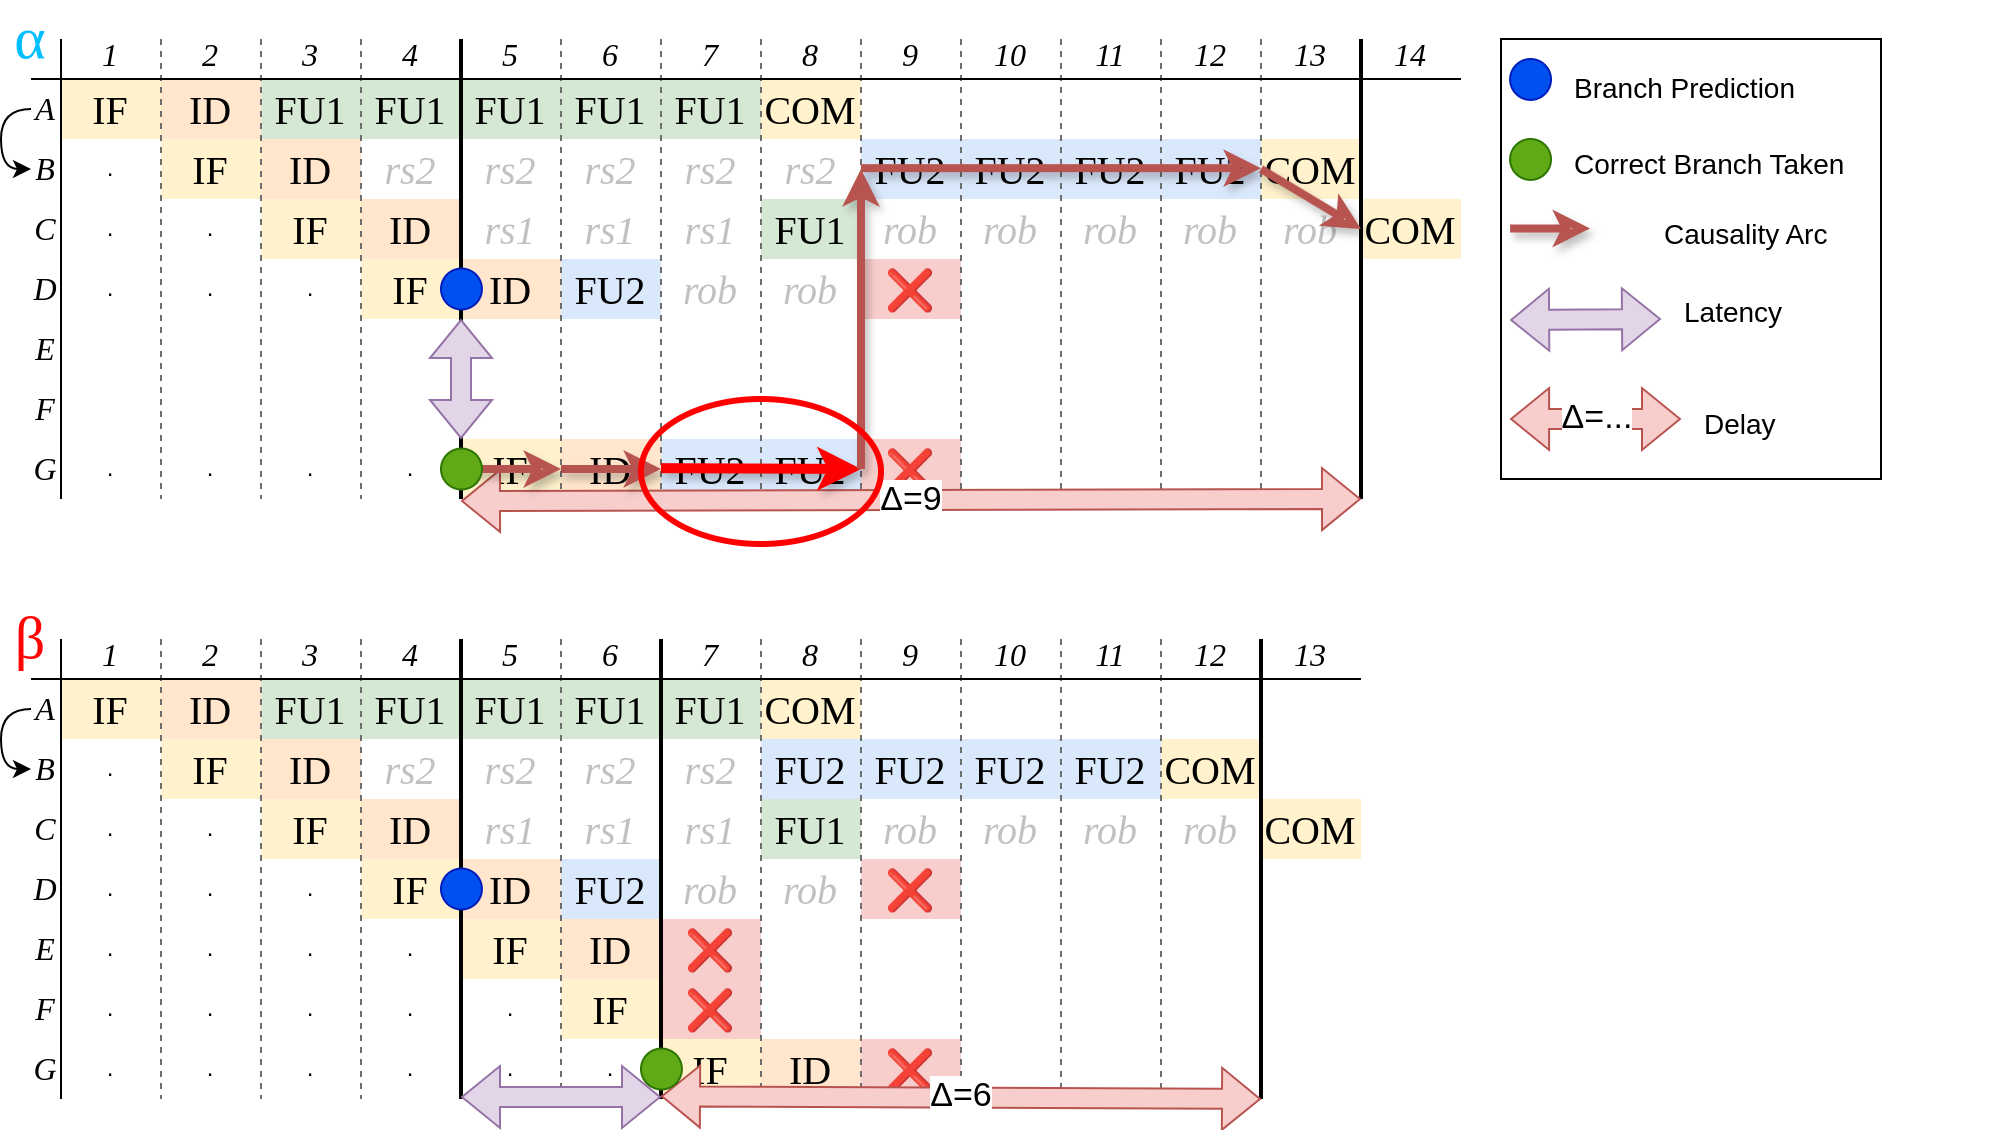
\includegraphics[width=0.9\textwidth]{pic/nested-bp-ta.png}
% \end{frame}


\begin{frame}[label=current]{FU release by FU acquisition}
    Where simple rules do not work.

    \includegraphics<1>[scale=0.13]{pic/nested-bp-ta-1.png}
    \includegraphics<2>[scale=0.13]{pic/nested-bp-ta-2.png}
    \includegraphics<3>[scale=0.13]{pic/nested-bp-ta-3.png}
    \includegraphics<4>[scale=0.13]{pic/nested-bp-ta-4.png}
    \includegraphics<5>[scale=0.13]{pic/nested-bp-ta-5.png}
    \includegraphics<6>[scale=0.13]{pic/nested-bp-ta-6.png}

    \begin{exampleblock}{"Acquisition" Rule}
        The FU acquisition is always causal to the respective FU release.
    \end{exampleblock}
\end{frame}
% make it bigger

\begin{frame}{FU release by squashing}
    \includegraphics<1>[scale=0.11]{pic/lat-mispred-1.png}
    \includegraphics<2>[scale=0.11]{pic/lat-mispred-2.png}
    \includegraphics<3>[scale=0.11]{pic/lat-mispred-3.png}
    \includegraphics<4>[scale=0.11]{pic/lat-mispred-4.png}
\end{frame}
% trace shorter

\begin{frame}
    Assumptions contradict each other!
\end{frame}

\begin{frame}{Results}
    \begin{itemize}
        \item The definition of Binder et al. can be applied in branch prediction context with minimal adjustments.
        \item Sometimes it is not evident which rule to use.
    \end{itemize}
\end{frame}

% Say that we have a bigger problem

\begin{frame}{Gap Problem}
    \includegraphics<1>[scale=0.17]{pic/gap-problem-1.png}
    \includegraphics<2>[scale=0.17]{pic/gap-problem-2.png}
    \includegraphics<3>[scale=0.17]{pic/gap-problem-3.png}
\end{frame}
% Make an animation

% \begin{frame}{Results}
%     \begin{itemize}
%         \item The definition of Binder et al. can be applied in branch prediction context with minimal adjustments.
%         \item Sometimes it is not evident which rule to use.
%         \item Initial definition suffers from a gap problem.
%         \item Likely, the problem is with causality itself.
%     \end{itemize}
% \end{frame}

% Results about assumptions -> to assumptions


\section{Conclusion}

\begin{frame}{Conclusion}
    \begin{itemize}
        \item Analyzed existing timing anomaly (TA) definitions; adopted Binder's causality-based approach.
        \item Developed a tool to systematically generate and analyze branch prediction-induced TAs.
        \item Binder's definition is adaptable, but controversial cases and a "gap problem" remain.
        \item Ongoing work: a new causality definition based on event constraints to address these issues.
        \item Future work: study the impact of branch predictor state.
    \end{itemize}
\end{frame}
% Add structure: results, future work


\end{document}
